% Options for packages loaded elsewhere
\PassOptionsToPackage{unicode}{hyperref}
\PassOptionsToPackage{hyphens}{url}
%
\documentclass[
]{book}
\usepackage{amsmath,amssymb}
\usepackage{iftex}
\ifPDFTeX
  \usepackage[T1]{fontenc}
  \usepackage[utf8]{inputenc}
  \usepackage{textcomp} % provide euro and other symbols
\else % if luatex or xetex
  \usepackage{unicode-math} % this also loads fontspec
  \defaultfontfeatures{Scale=MatchLowercase}
  \defaultfontfeatures[\rmfamily]{Ligatures=TeX,Scale=1}
\fi
\usepackage{lmodern}
\ifPDFTeX\else
  % xetex/luatex font selection
\fi
% Use upquote if available, for straight quotes in verbatim environments
\IfFileExists{upquote.sty}{\usepackage{upquote}}{}
\IfFileExists{microtype.sty}{% use microtype if available
  \usepackage[]{microtype}
  \UseMicrotypeSet[protrusion]{basicmath} % disable protrusion for tt fonts
}{}
\makeatletter
\@ifundefined{KOMAClassName}{% if non-KOMA class
  \IfFileExists{parskip.sty}{%
    \usepackage{parskip}
  }{% else
    \setlength{\parindent}{0pt}
    \setlength{\parskip}{6pt plus 2pt minus 1pt}}
}{% if KOMA class
  \KOMAoptions{parskip=half}}
\makeatother
\usepackage{xcolor}
\usepackage{longtable,booktabs,array}
\usepackage{calc} % for calculating minipage widths
% Correct order of tables after \paragraph or \subparagraph
\usepackage{etoolbox}
\makeatletter
\patchcmd\longtable{\par}{\if@noskipsec\mbox{}\fi\par}{}{}
\makeatother
% Allow footnotes in longtable head/foot
\IfFileExists{footnotehyper.sty}{\usepackage{footnotehyper}}{\usepackage{footnote}}
\makesavenoteenv{longtable}
\usepackage{graphicx}
\makeatletter
\def\maxwidth{\ifdim\Gin@nat@width>\linewidth\linewidth\else\Gin@nat@width\fi}
\def\maxheight{\ifdim\Gin@nat@height>\textheight\textheight\else\Gin@nat@height\fi}
\makeatother
% Scale images if necessary, so that they will not overflow the page
% margins by default, and it is still possible to overwrite the defaults
% using explicit options in \includegraphics[width, height, ...]{}
\setkeys{Gin}{width=\maxwidth,height=\maxheight,keepaspectratio}
% Set default figure placement to htbp
\makeatletter
\def\fps@figure{htbp}
\makeatother
\setlength{\emergencystretch}{3em} % prevent overfull lines
\providecommand{\tightlist}{%
  \setlength{\itemsep}{0pt}\setlength{\parskip}{0pt}}
\setcounter{secnumdepth}{5}
\usepackage{booktabs}
\ifLuaTeX
  \usepackage{selnolig}  % disable illegal ligatures
\fi
\usepackage[]{natbib}
\bibliographystyle{plainnat}
\IfFileExists{bookmark.sty}{\usepackage{bookmark}}{\usepackage{hyperref}}
\IfFileExists{xurl.sty}{\usepackage{xurl}}{} % add URL line breaks if available
\urlstyle{same}
\hypersetup{
  pdftitle={AI Declassified: A Ross Faculty Survival Guide},
  pdfauthor={Adam Zhang, Ryan Berger, Michelle Xu, Fuad Chedid, Sona Coshal},
  hidelinks,
  pdfcreator={LaTeX via pandoc}}

\title{AI Declassified: A Ross Faculty Survival Guide}
\author{Adam Zhang, Ryan Berger, Michelle Xu, Fuad Chedid, Sona Coshal}
\date{2023-08-16}

\begin{document}
\maketitle

{
\setcounter{tocdepth}{1}
\tableofcontents
}
\hypertarget{introduction}{%
\chapter{Introduction}\label{introduction}}

In an era of rapid technological advancement, Artificial Intelligence stands as a transformative force with the potential to reshape academia. Generative AI---driven by cutting-edge models like OpenAI's GPT-3---has demonstrated remarkable capabilities in a diverse array of applications, ranging from natural language generation to content creation, problem-solving, and even creative arts. As we stand at the base of a technological revolution that will reshape many aspects of humanity, it becomes imperative to assess its potential ramifications within the context of higher education. This analysis explores how generative AI will influence education at the Stephen M. Ross School of Business---focusing on its impact on the school's faculty and staff. Our project begins by examining generative AI's current capabilities and real-world uses. We explored a multitude of AI-driven content generation, seeing it firsthand and exploring its implications for fostering innovation and efficiency across a wide range of both creative and more structured disciplines.

Faculty interviews provide a comprehensive range of perspectives, from optimism to caution, highlighting its potential to reshape the traditional role of teaching, redefine teacher-student relationships, and rethink what should be prioritized in educating business leaders of the future. By tapping into the collective wisdom of our esteemed faculty, we sought to uncover insights and current perspectives on the use of generative AI, considering its role in curriculum, academic integrity, and its overall implications for the future of education at the Ross School of Business. These conversations spanned a range of perspectives, from cautious optimism to enthusiastic embrace for its potential.

We also assess university policies, providing a backdrop for evaluating generative AI adoption. By critically analyzing the existing guidelines and resources within the University of Michigan, we aim to shed light on the regulatory framework within which our university will operate into the foreseeable future. Some examples of such are the Generative AI Advisory (GAIA) Committee and the creation of a UMich-based ChatGPT competitor for potential use within the university. This assessment serves as a crucial backdrop against which we evaluate the potential opportunities and challenges associated with generative AI adoption.

Our project concludes by distilling faculty insights, university policies, and current applications of generative AI into practical recommendations---guiding our faculty to leverage AI's potential while addressing ethical, pedagogical, and general institutional considerations. In summation, this serves as a guide through generative AI's impact on business education, providing a roadmap for faculty members to navigate the ever-evolving landscape with insight, foresight, and adaptability. By embracing the power of generative AI, the Ross School of Business has the potential to enhance, enrich, and modernize the educational experience of current and future students.

\hypertarget{about-us}{%
\chapter{About Us}\label{about-us}}

We are a dynamic team of aspiring business analysts pursuing our Master's in Business Analytics. With a passion for extracting value from data, we strive to make a tangible impact by delivering innovative solutions and optimizing strategies. In this project, we utilized our diverse set of backgrounds and experiences to create a project surrounding the implications of AI at Ross. We aim to deliver a product that assists both faculty, staff, and students like ourselves that are faced with the challenges of integrating AI into our education and everyday lives. Here is a little bit about each of us!

\hypertarget{ryan-berger}{%
\section{Ryan Berger}\label{ryan-berger}}

Hey! I'm Ryan Berger. I am a current Master's of Business Analytics student at Michigan Ross. In my undergrad, I also attended Michigan through the School of Information, studying data analytics. I am from New Jersey, which means I am a Giants fan and I like to say I'm from New York. Go Blue!

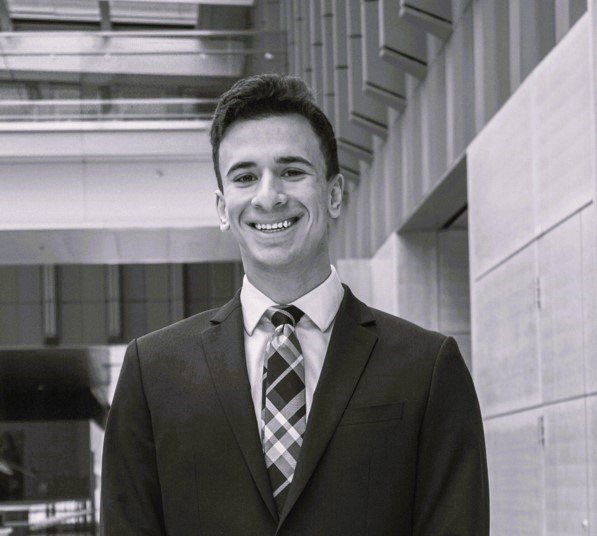
\includegraphics[width=0.4\linewidth]{rtberger}

\hypertarget{adam-zhang}{%
\section{Adam Zhang}\label{adam-zhang}}

Hi! I'm Adam Zhang. I am a Master of Business Analytics student at the Ross School of Business at University of Michigan. I attended University of Illinois Urbana-Champaign where I majored economics for undergrad. I enjoy cooking, watching movies, listening to musics (mainly 70s and 80s), and going to art museums.

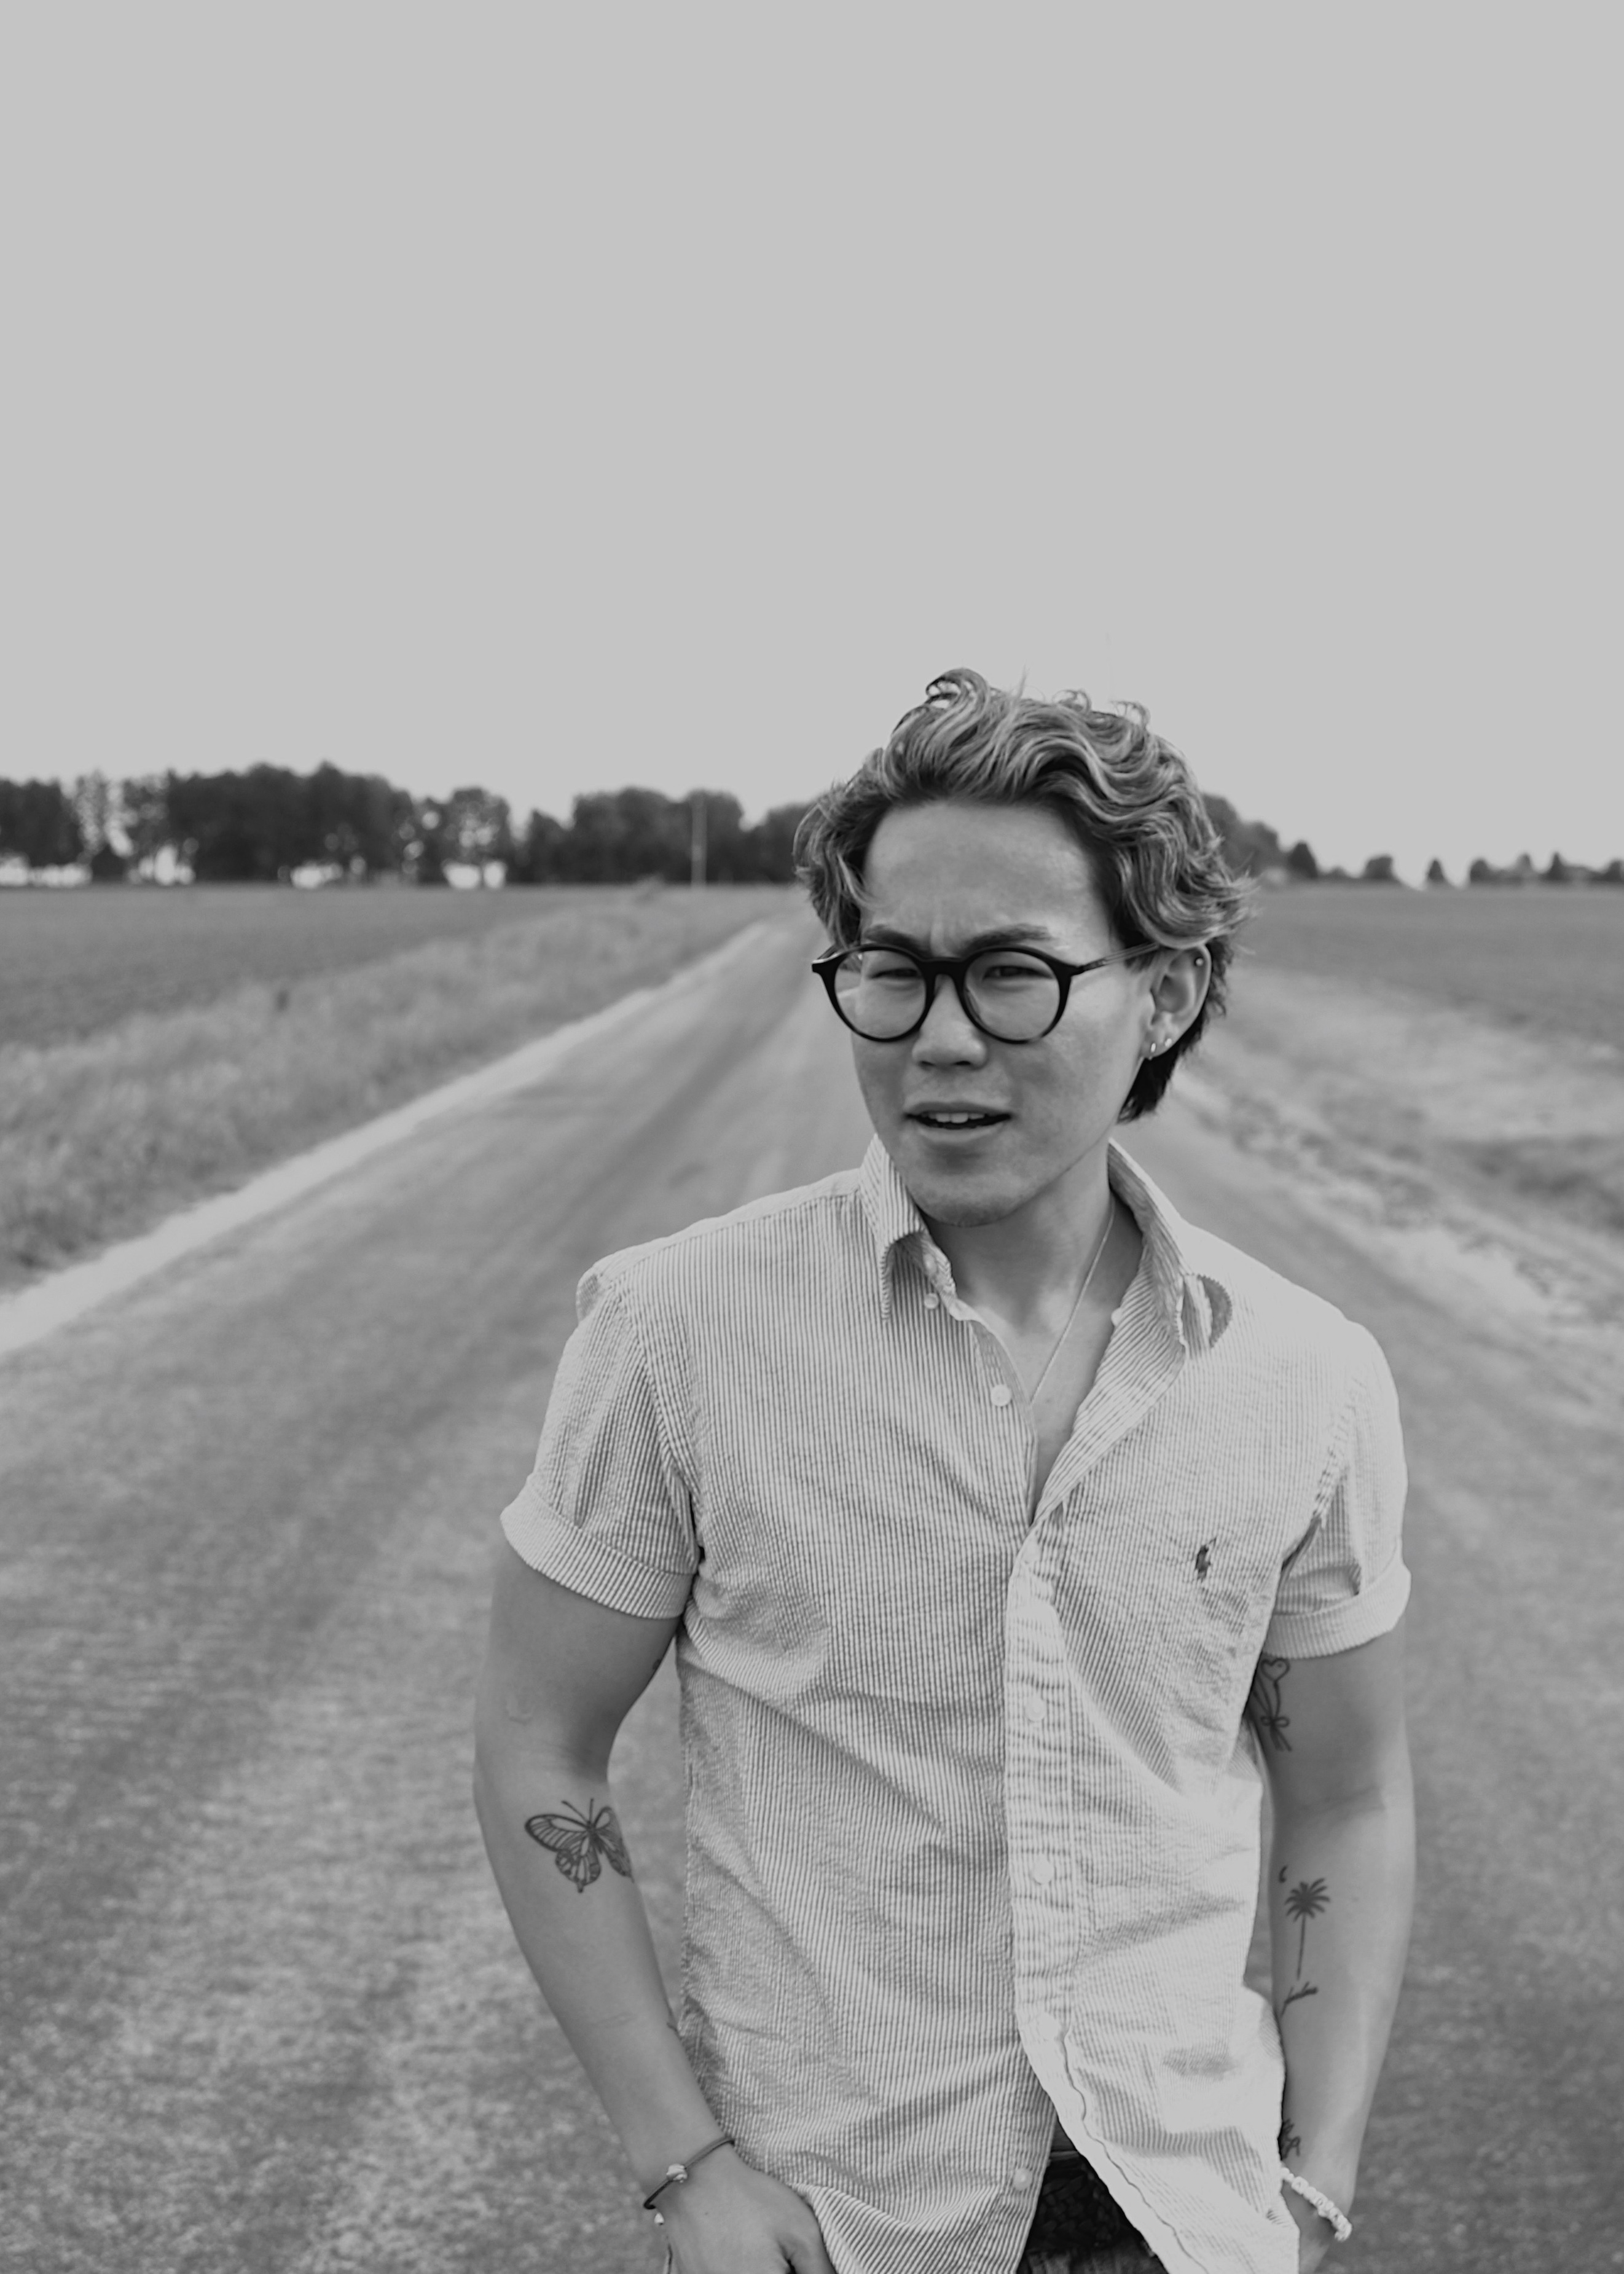
\includegraphics[width=0.4\linewidth]{AZ}

\hypertarget{michelle-xu}{%
\section{Michelle Xu}\label{michelle-xu}}

Hello, I'm Michelle Xu, originally from China. I spent six years living in the beautiful city of San Diego, California. After high school, I moved to Ann Arbor, Michigan, to pursue a major in Bioinformatics at LS\&A. Currently, I'm a Master of Business Analytics student at the University of Michigan, Ross School of Business.

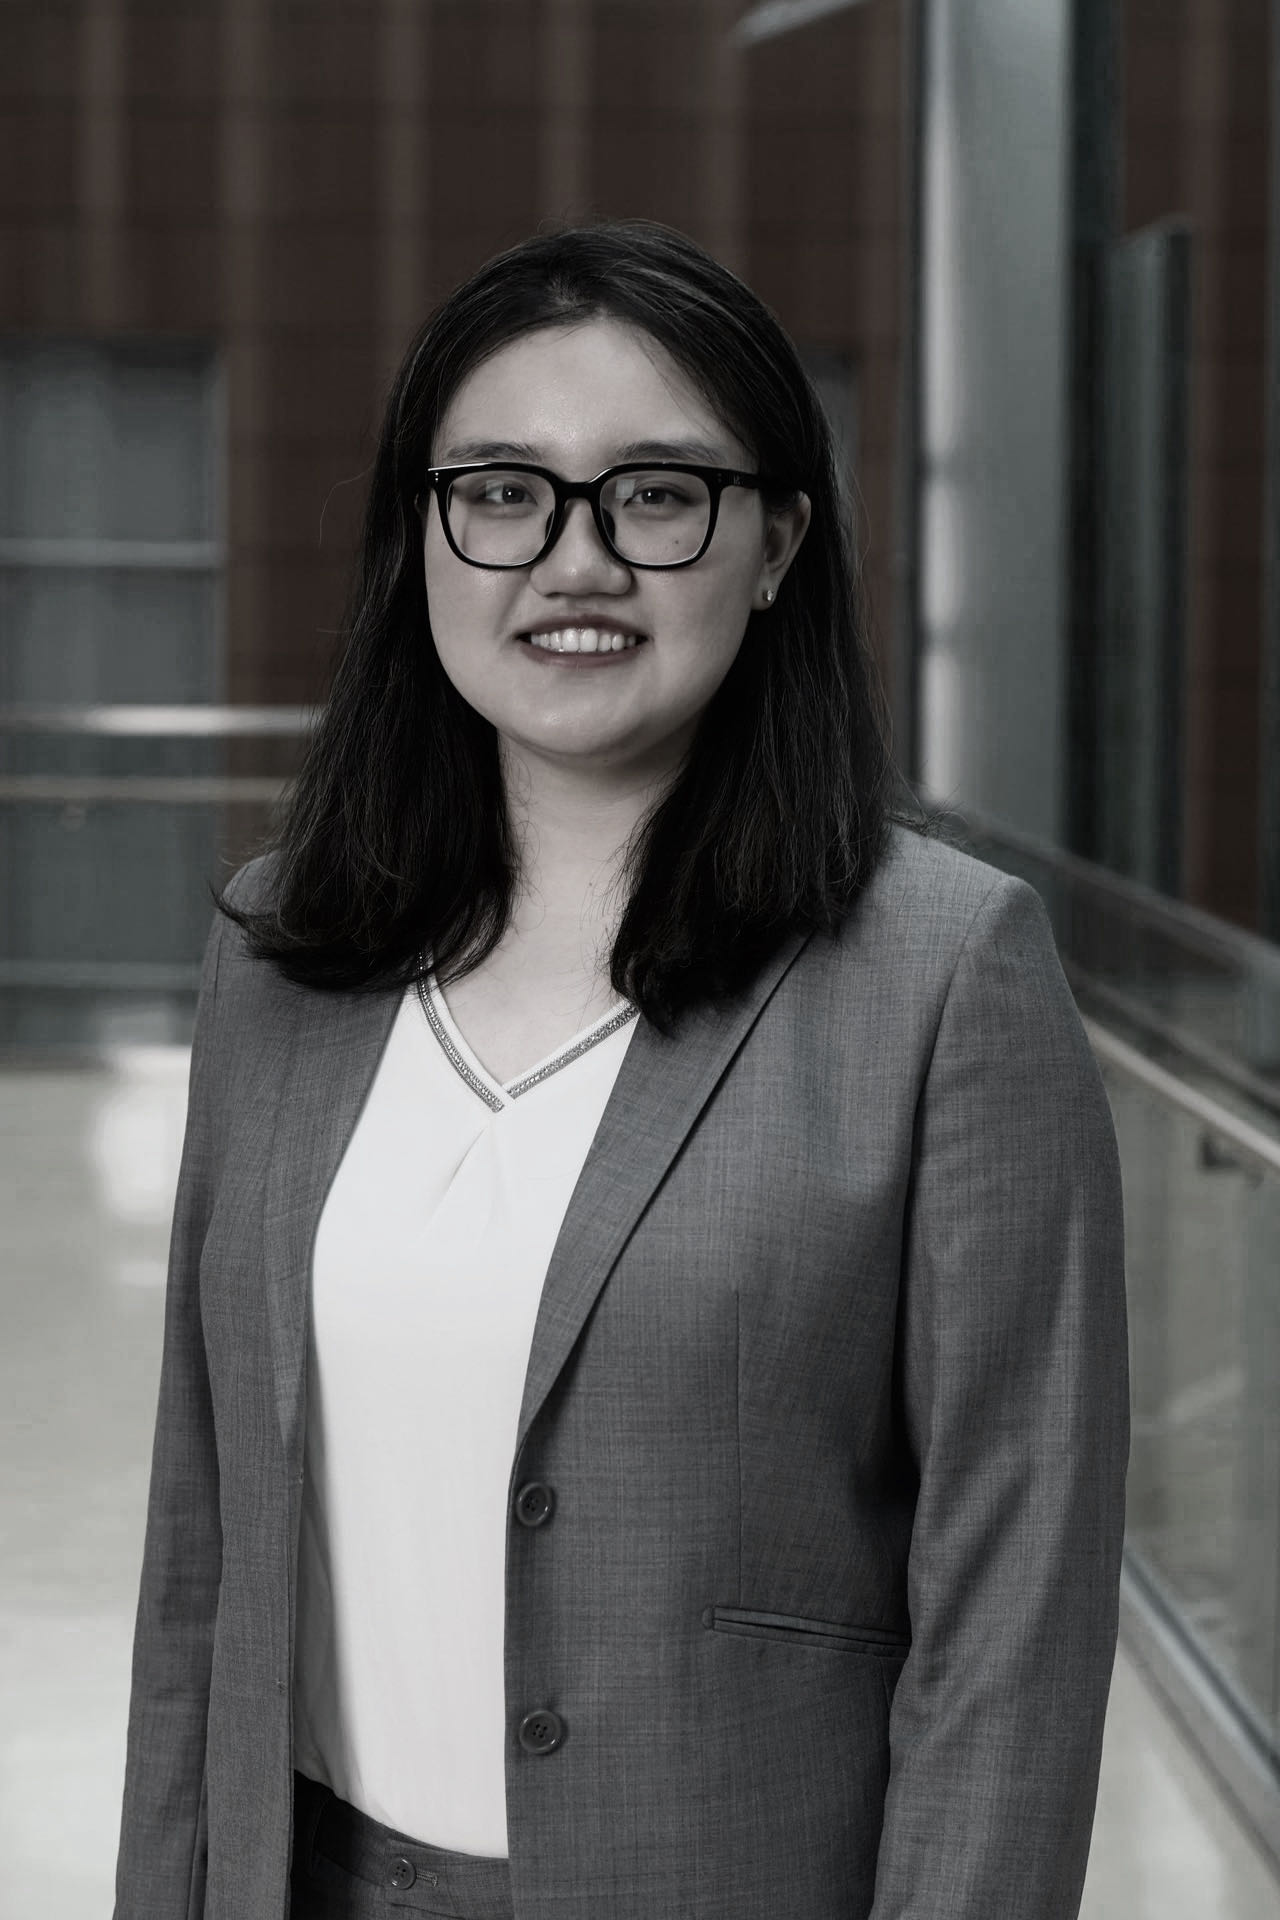
\includegraphics[width=0.4\linewidth]{WechatIMG10}

\hypertarget{sona-coshal}{%
\section{Sona Coshal}\label{sona-coshal}}

Hi, my name is Sona! I'm born and raised in Columbia, South Carolina and a proud USC Gamecock! I have a BSBA in Finance and Supply Chain from the Darla Moore School Business.

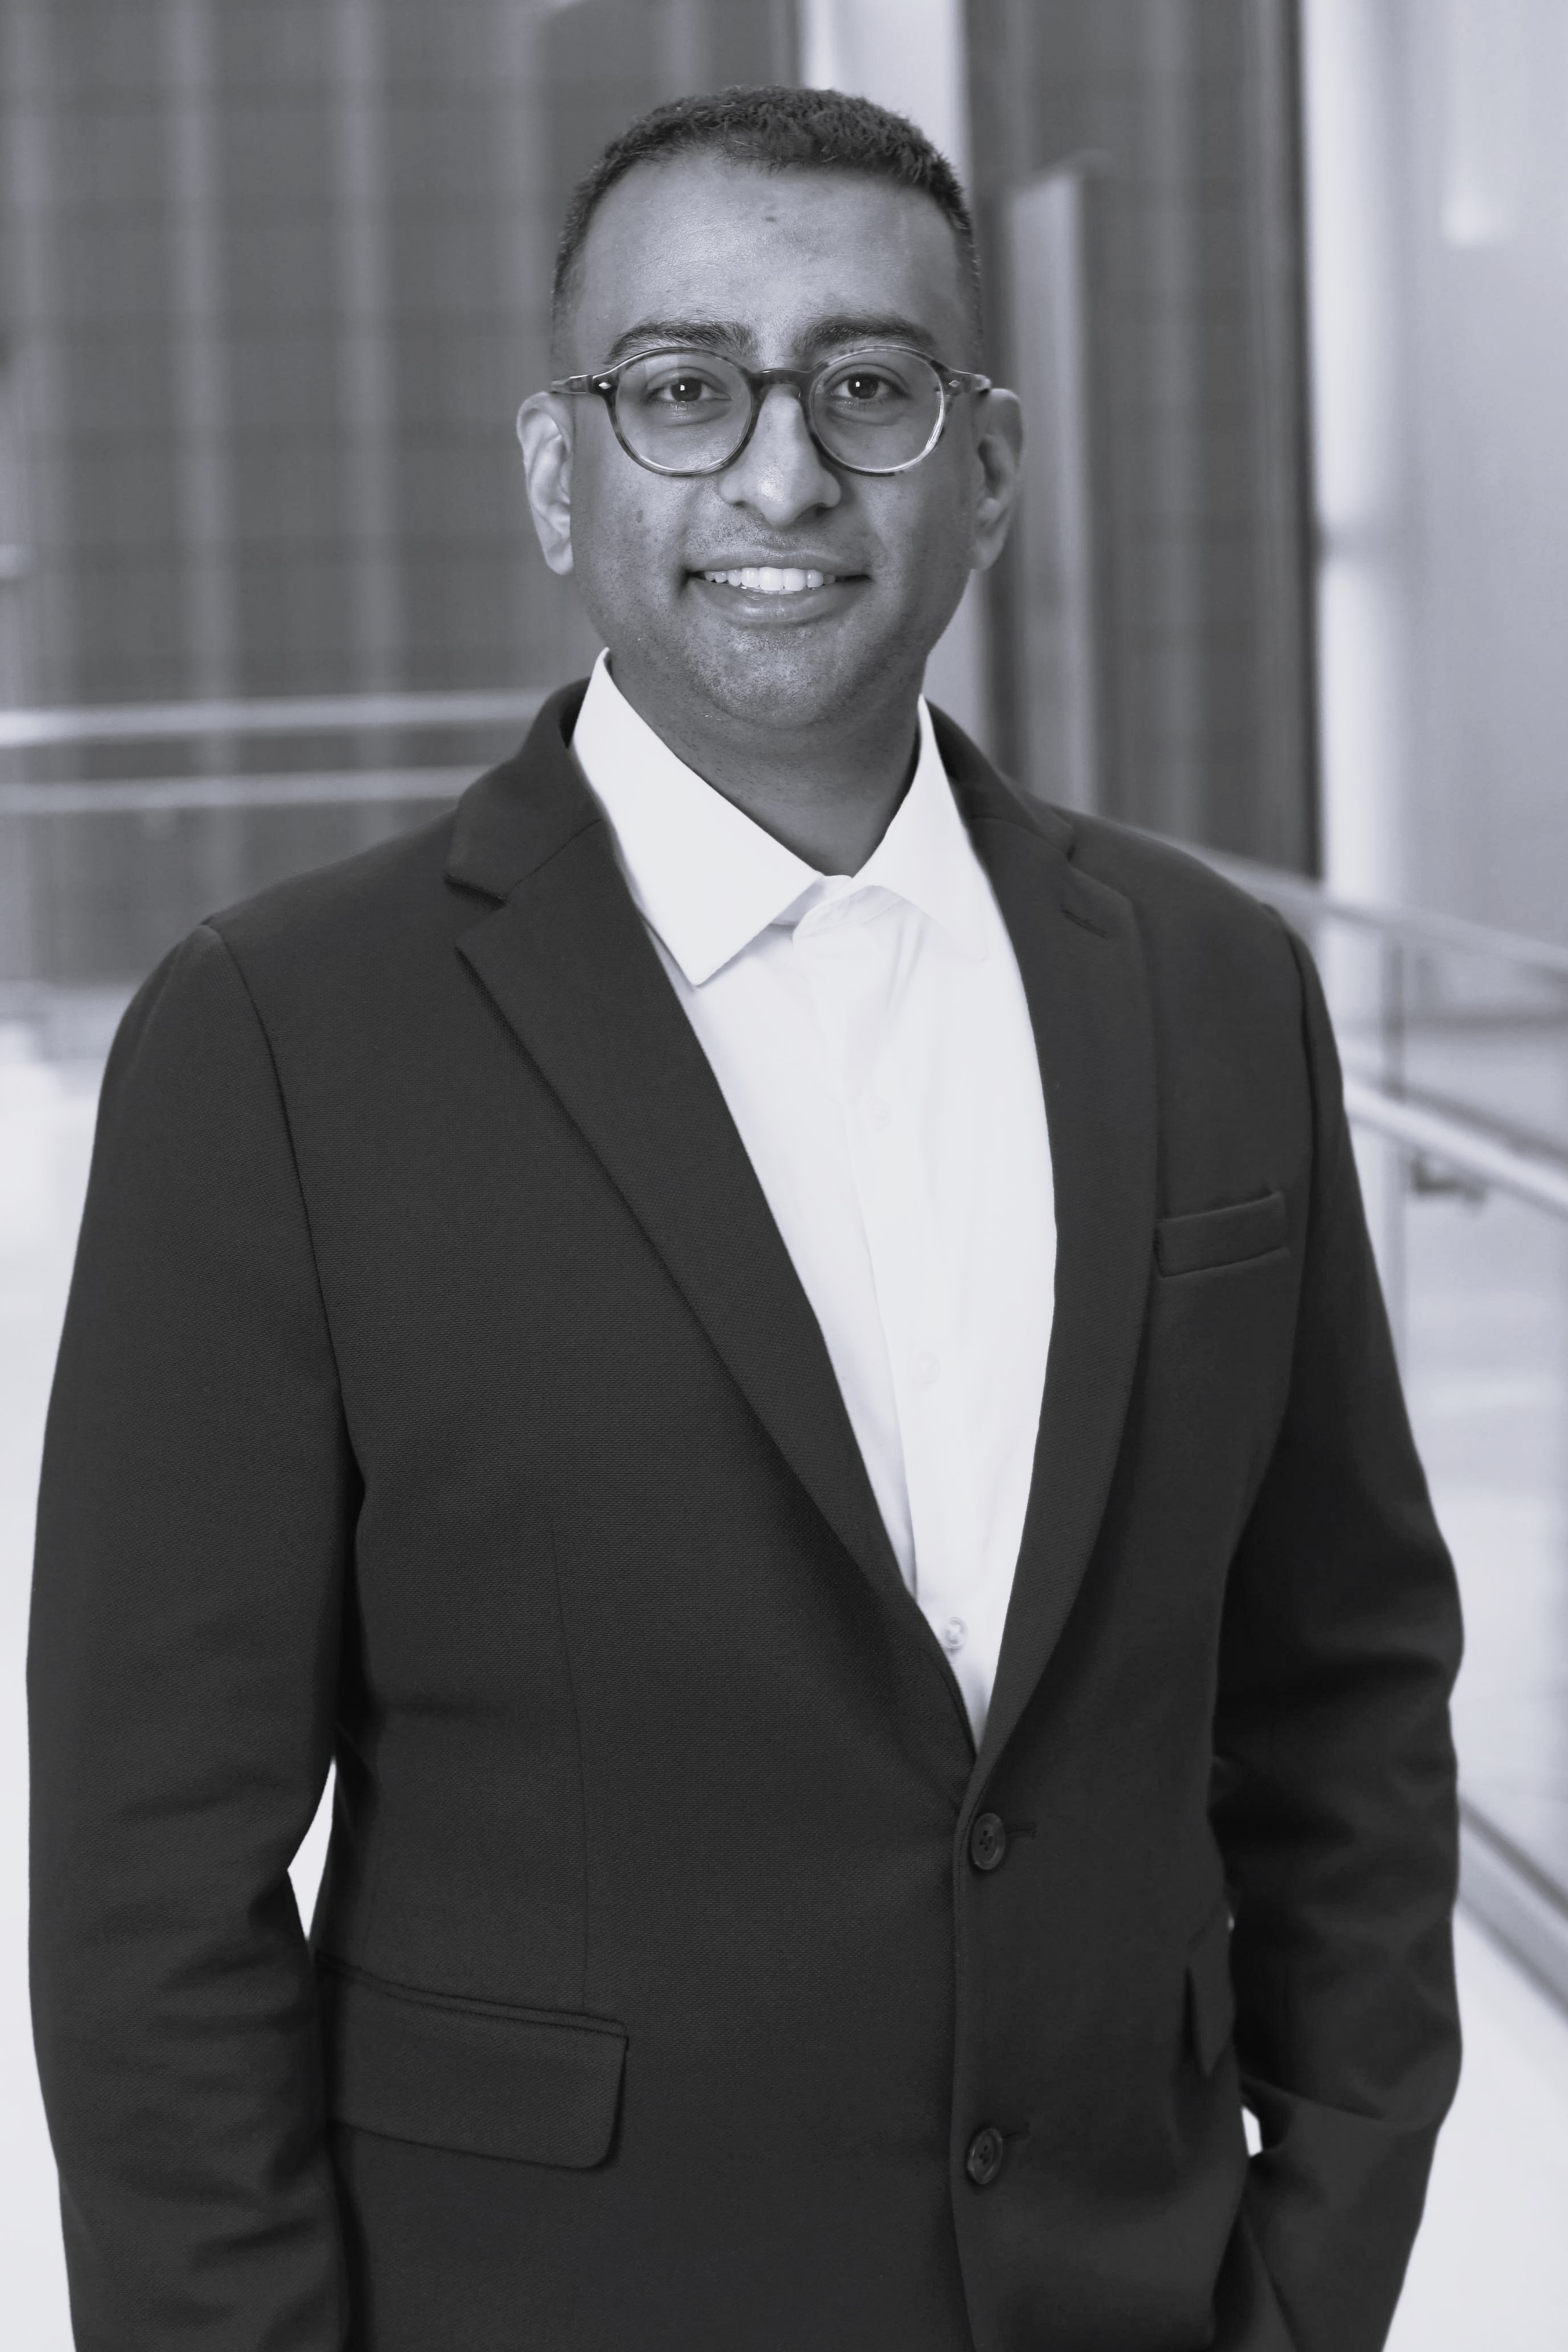
\includegraphics[width=0.4\linewidth]{Sona's_Photo}

\hypertarget{fuad-chedid}{%
\section{Fuad Chedid}\label{fuad-chedid}}

Hi! I'm Fuad, a native Michigander! Before joining the Master of Business Analytics program at Michigan Ross, I was based in Dubai, UAE, and worked in the energy sector. I consider myself a ``tech head'' and my main area of interest is the intersection of business and technology. I enjoy travelling and so far have visited 27 countries and five continents.

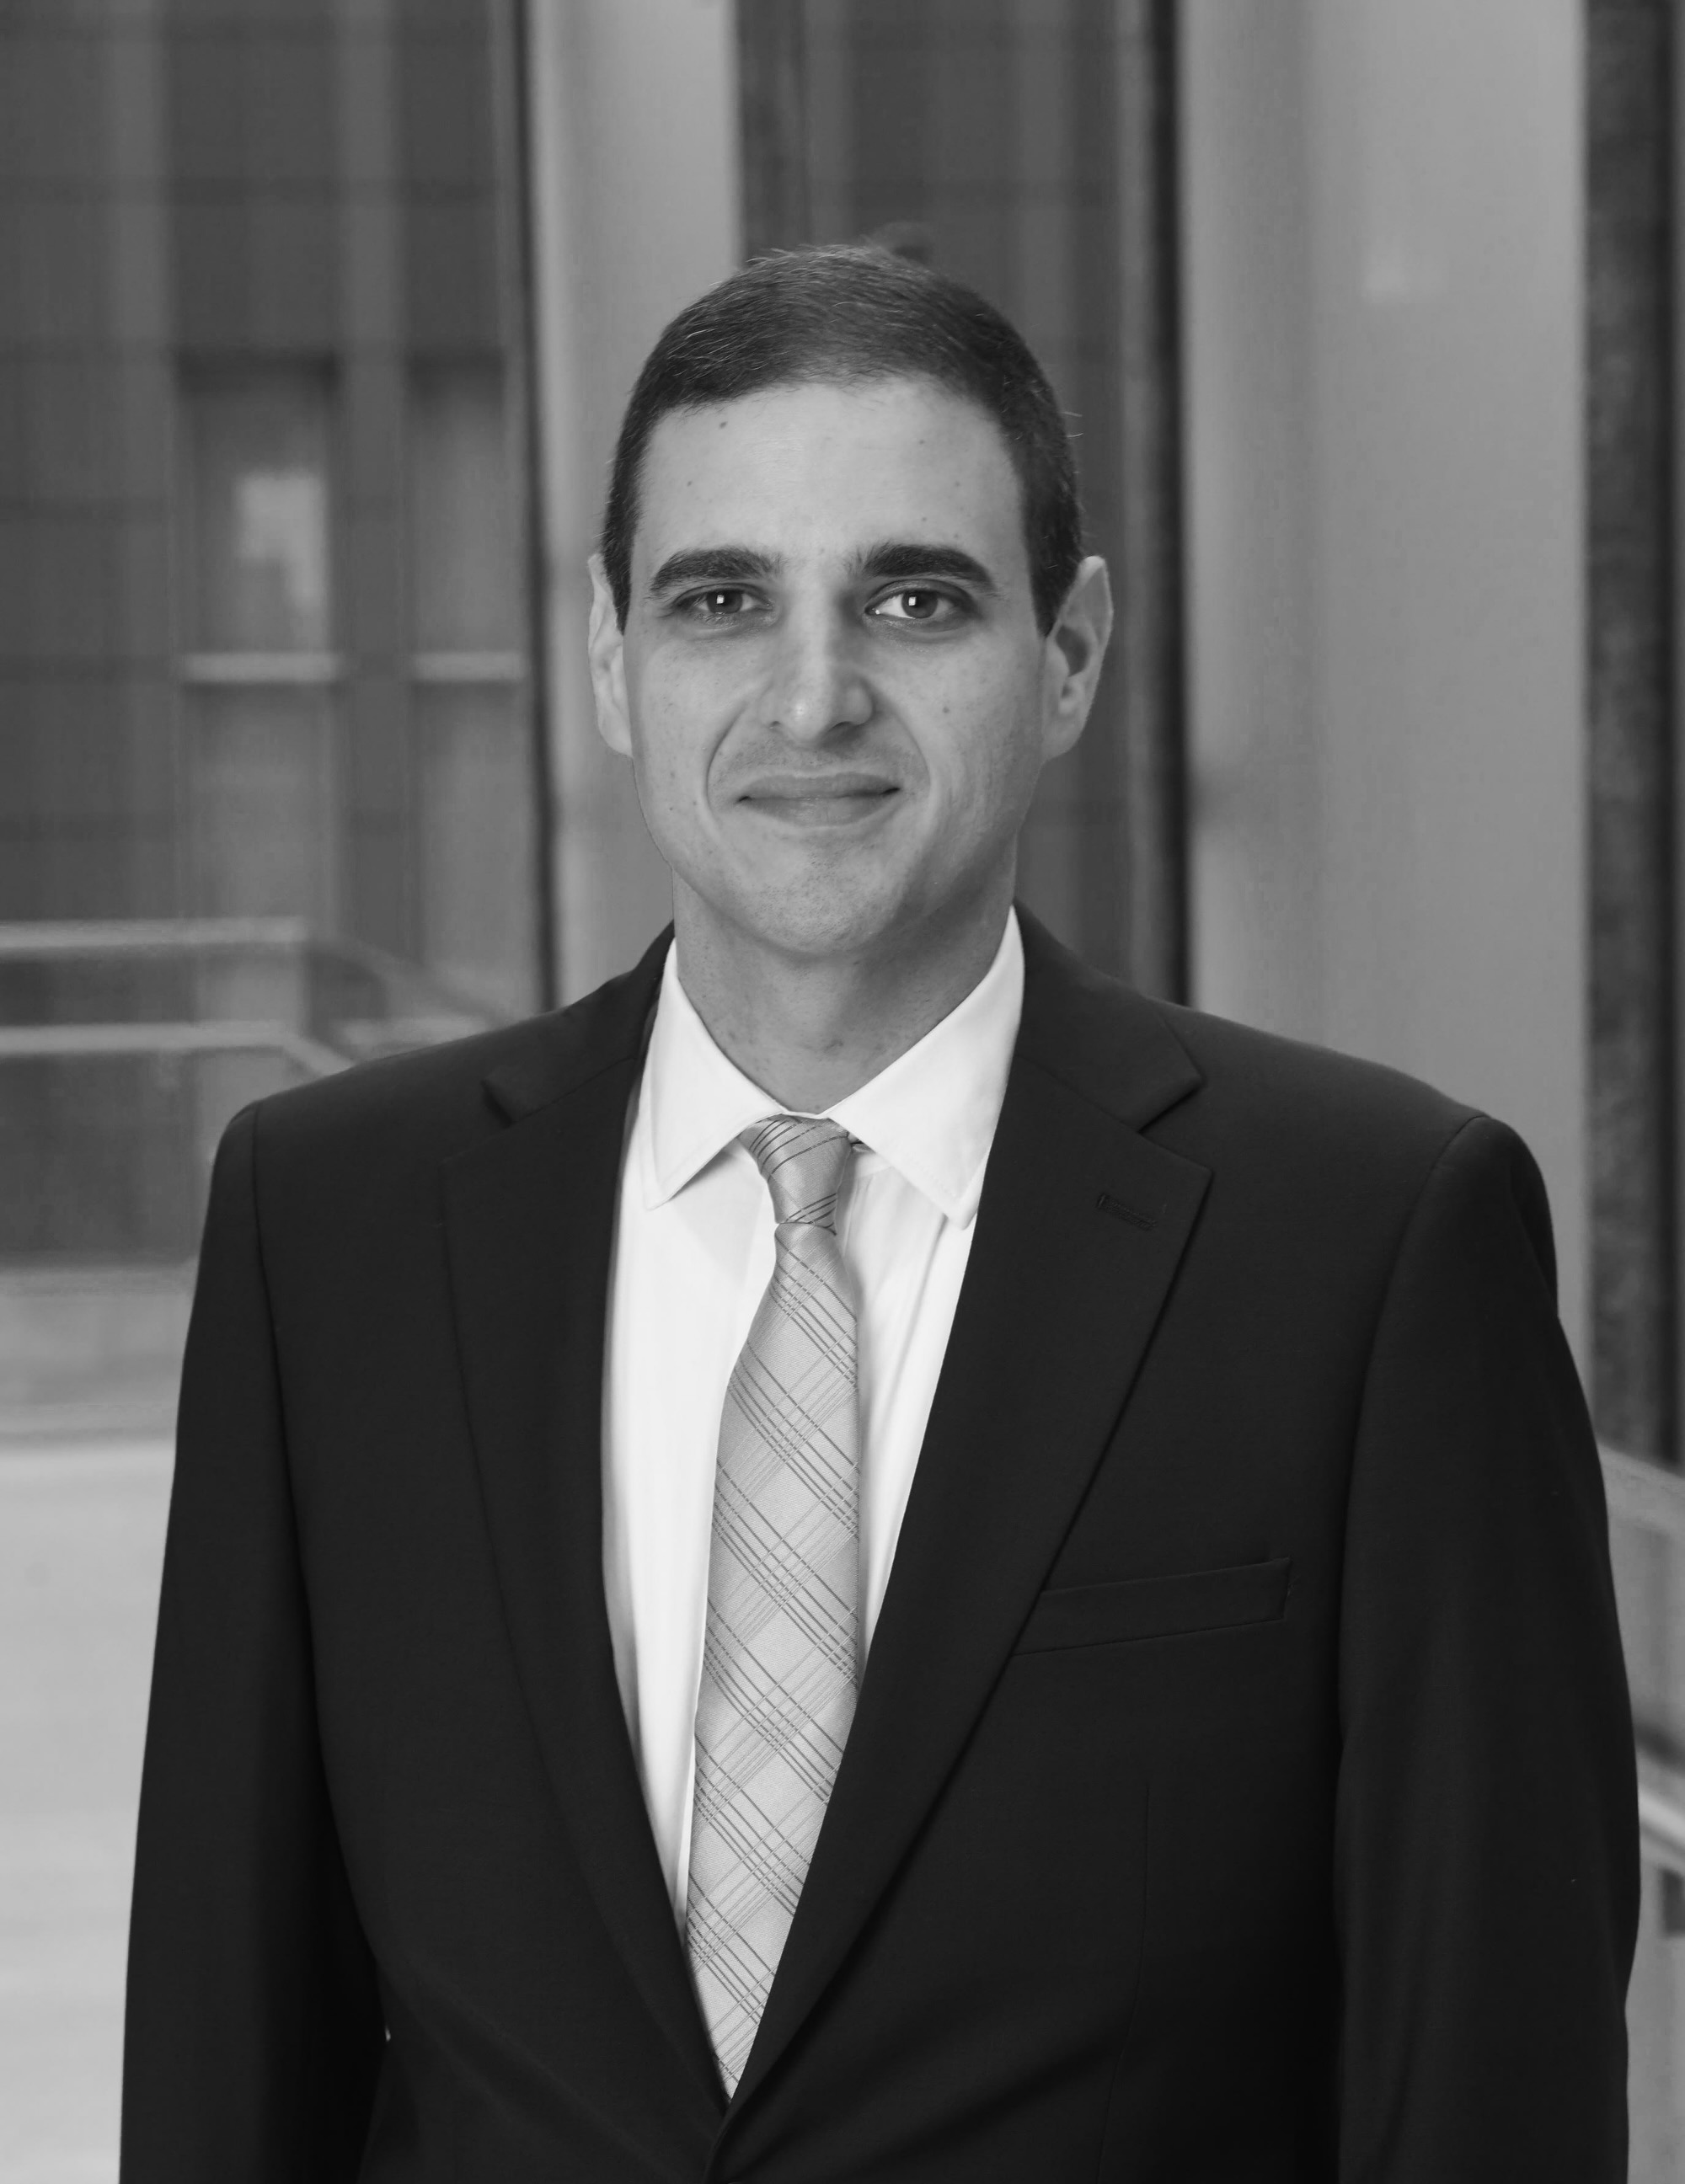
\includegraphics[width=0.4\linewidth]{fpic}

\hypertarget{current-state-of-affairs}{%
\chapter{Current State of Affairs}\label{current-state-of-affairs}}

Since the proliferation of publicly available generative AI in November 2022, U-M has been positioning itself to respond and adapt. Undoubtedly, there is a need for institutional understanding and action to ensure that generative AI is leveraged in support of the University's mission. This section provides information on the currently published university-wide guidance.

\hypertarget{u-m-genai-website}{%
\section{U-M GenAI Website}\label{u-m-genai-website}}

Recently established by the GAIA Committee (see \ref{gaia-committee}), \url{https://genAI.umich.edu} is a comprehensive resource containing the latest guidance and information for all members of the U-M community.

\hypertarget{gaia-committee}{%
\section{GAIA Committee}\label{gaia-committee}}

The Generative AI Advisory (\href{https://it.umich.edu/strategy-planning/gaia}{GAIA}) Committee was established in the first half of 2023, with the overall aim being:

\begin{quote}
``to provide guidance to the university community for the use of generative AI and provide strategic advice to the~VPIT-CIO~and Provost.''
\end{quote}

An overview of the committee's \href{https://genai.umich.edu/committee-report}{official report}, published on June 30th 2023, is provided in section \ref{initial-report-june-30-2023}.

The committee currently includes members from the following schools, colleges, and departments:

\begin{longtable}[]{@{}ll@{}}
\toprule\noalign{}
School / College / Department & \# of Member(s) \\
\midrule\noalign{}
\endhead
\bottomrule\noalign{}
\endlastfoot
\textbf{Executive Sponsor} & 1 \\
\textbf{College of Engineering} & 4 \\
\textbf{Medical School} & 2 \\
\textbf{School of Public Health} & 1 \\
\textbf{College of Literature, Science, and the Arts} & 3 \\
\textbf{School of Education} & 2 \\
\textbf{School of Information} & 2 \\
\textbf{Ross School of Business} & 2 \\
\textbf{Information and Technology Services} & 1 \\
\textbf{Center for Research on Learning and Teaching} & 1 \\
\textbf{Center for Academic Innovation} & 1 \\
\textbf{Office of the Provost for DE\&I} & 1 \\
\textbf{U-M Flint} & 1 \\
\textbf{U-M Dearborn} & 1 \\
\end{longtable}

\emph{As of Aug 2023. Note: Some members represent more than one affiliation.}

\hypertarget{initial-report-june-30-2023}{%
\subsection{Initial Report (June 30 2023)}\label{initial-report-june-30-2023}}

The below extracts from the \href{https://genai.umich.edu/committee-report}{report} have been selectively chosen based on their immediate relevancy to instructors.

\hypertarget{overall-recommendations}{%
\subsubsection*{Overall Recommendations}\label{overall-recommendations}}
\addcontentsline{toc}{subsubsection}{Overall Recommendations}

A brief highlight of the overarching recommendations:


\includegraphics[width=0.3125in,height=0.20833in]{open.png}

\begin{quote}
\begin{itemize}
\item
  Dissemination of guidance and launch of campus discussion (Timeline: immediate).
\item
  Teaching, Learning, and Academic Innovation (Timeline: Fall 2023). U-M can approach GenAI as an opportunity to rethink how we teach and define meaningful learning objectives, promote inclusion and equity, and assess learning. \textbf{Instructors should be given complete flexibility to allow or disallow the use of GenAI tools.}
\item
  Assess the use of GenAI in research and set best practice standards for privacy protections; data use controls; and updating research integrity reated SPGs, PEERS modules, and RCR training.
\item
  Provost, VPR and VPIT should establish a U-M wide research initiative in the area of Generative AI (Timeline: Fall 2023/Winter 2024).

  \begin{itemize}
  \tightlist
  \item
    U-M should consider developing its own version of foundation GenAI models to enable research and innovation (Timeline: Begin activities in Fall 2023).
  \end{itemize}
\item
  Expansion of IT infrastructure to accommodate secure and equitable access to GenAI plat- forms and tools (Timeline: Immediate and Variable).

  \begin{itemize}
  \tightlist
  \item
    Create and deliver new GenAI services. These services will be offered across three tiers, each catering to different needs and technical proficiencies and made available to Ann Arbor, Flint, and Dearborn.
  \end{itemize}
\item
  VPIT to work with the GAIA committee to coordinate and establish an AI digital commons where our community can share best practices and emerging ideas in GenAI (Timeline: Immediate).
\item
  Launch a U-M GenAI website providing strategy, policies, resources, and links. Coordinate this with a well-defined communication plan (Timeline: Immediate).
\end{itemize}
\end{quote}


\includegraphics[width=0.3125in,height=0.20833in]{close.png}

\hypertarget{key-benefits-and-opportunities}{%
\subsubsection*{Key Benefits and Opportunities}\label{key-benefits-and-opportunities}}
\addcontentsline{toc}{subsubsection}{Key Benefits and Opportunities}

Highlights of key benefits and opportunities:


\includegraphics[width=0.3125in,height=0.20833in]{open.png}

\begin{quote}
\begin{itemize}
\item
  GenAI will enable U-M to advance its mission and accelerate and support Vision 2034.
\item
  GenAI has the potential to transform teaching outcomes by creating customizable learning pathways
\item
  GenAI will accelerate knowledge development,including rethinking of disciplinary boundaries and domains, and possibly, defining new ones.
\item
  From an efficiency perspective, GenAI has the potential to support enhanced administrative productivity and service quality throughout the University.
\item
  \textbf{U-M has the intellectual depth, resources, and international and national connections and networks to be the leader in the development and appropriate use of GenAI.}
\end{itemize}
\end{quote}


\includegraphics[width=0.3125in,height=0.20833in]{close.png}

\hypertarget{key-threats-and-weaknesses}{%
\subsubsection*{Key Threats and Weaknesses}\label{key-threats-and-weaknesses}}
\addcontentsline{toc}{subsubsection}{Key Threats and Weaknesses}

Highlights of key threats and weaknesses:


\includegraphics[width=0.3125in,height=0.20833in]{open.png}

\begin{quote}
\begin{itemize}
\item
  Several technical weaknesses currently exist, including temporal ignorance, hallucination and fabrication, misattribution, overriding safety protocols, inadvertent inclusion breaches or ethical problems, and bias in training data.
\item
  Social weaknesses refer to those that arise from the interaction between the system and user, which may yield unanticipated actions and outcomes. While myriad and evolving, a few examples of social weaknesses include

  \begin{itemize}
  \item
    rapid escalation of deep fakes in video and audio,
  \item
    user attribution of output generated by GenAI to themselves or others,
  \item
    GenAI companion giving dangerous advice to children,
  \item
    use of GenAI to perform research without appropriate disclosure,
  \item
    inappropriate use of prompt data by AI provider,
  \item
    reduced demand for human labor in many professions,
  \item
    inequitable access to state-of-the-art GenAI systems,
  \item
    and unauthorized generation or replication of copyrighted or otherwise protected material.
  \end{itemize}
\end{itemize}
\end{quote}


\includegraphics[width=0.3125in,height=0.20833in]{close.png}

\hypertarget{instructor-recommendations}{%
\subsubsection*{Instructor Recommendations}\label{instructor-recommendations}}
\addcontentsline{toc}{subsubsection}{Instructor Recommendations}

The committee's initial report identifies teaching and learning as the most \emph{``immediate and significant GenAI application domain''} and provides guidance to instructors to help prepare for the Fall 2023 semester. The below sections include highlights of the guidance.

Generally, the committee finds that it is presently ``nearly impossible to enforce'' banning GenAI use in coursework. And therefore, strongly recommends that instructors consider the following questions when adapting course work:


\includegraphics[width=0.3125in,height=0.20833in]{open.png}

\begin{quote}
\begin{itemize}
\item
  Should GenAI be used in the course or not---and why or why not?
\item
  If GenAI is to be used, how is the use to be documented?
\item
  Should course learning objectives be revised?
\item
  Should GenAI competencies be taught in the specific disciplinary context?
\item
  Should assessments be revised?
\end{itemize}
\end{quote}


\includegraphics[width=0.3125in,height=0.20833in]{close.png}

\hypertarget{genai-permit-or-ban}{%
\paragraph*{GenAI: permit or ban?}\label{genai-permit-or-ban}}
\addcontentsline{toc}{paragraph}{GenAI: permit or ban?}

The report also addresses the fact that current academic misconduct definitions, Honor Codes, and academic integrity policies do not account for GenAI explicitly, and should be updated. The committee also acknowledges that students who use GenAI in an unauthorized manor may be committing cheating or plagiarism.

In determining GenAI permissability within academic misconduct policies, the report provides the following view:


\includegraphics[width=0.3125in,height=0.20833in]{open.png}

\begin{quote}
Common approaches to updating academic misconduct policies are:

\begin{itemize}
\item
  Determining that ChatGPT (or GenAI) is prohibited help from another ``person'' (e.g., UCLA),
\item
  Defining GenAI as a ``source'' that should be acknowledged (e.g., UW Madison).
\end{itemize}

The GAIA committee believes that the ``person'' approach misleadingly attributes sentience and a reasoning capacity to GenAI, and proposes that the ``source'' approach is more workable, and aligned with our mission of teaching students to engage effectively and ethically with the world around them.
\end{quote}


\includegraphics[width=0.3125in,height=0.20833in]{close.png}

With regard to course policy, the report provides the following guidance to instructors:


\includegraphics[width=0.3125in,height=0.20833in]{open.png}

\begin{quote}
\begin{itemize}
\item
  it is critical that expectations are clearly articulated in the syllabus and continually reinforced when assignments are given.
\item
  \textbf{instructors should be given flexibility to allow or disallow the use of GenAI tools. If the latter approach is adopted, the committee discourages the use of surveillance and plagiarism detection tools as they cannot be reliably counted upon at the present moment.}
\item
  GenAI is changing rapidly, and new tools will become available. Course policies therefore need to be provisional and subject to change.
\end{itemize}

Course policies might fall into one of three categories:

\begin{itemize}
\item
  Specific uses of GenAI are encouraged (generating ideas, editing, translating, outlining).
\item
  Specific uses of GenAI are allowed if students clearly distinguish between their original work and GenAI output (highlighting output, tracking changes in GenAI output).
\item
  Any use of GenAI constitutes academic misconduct.
\end{itemize}

If GenAI tools are allowed, the instructor should be clear which tools are allowed and in what capacity. On the other hand, if GenAI tools are disallowed, the committee suggests that the instructor give reasons why the use of GenAI tools would hinder learning.
\end{quote}


\includegraphics[width=0.3125in,height=0.20833in]{close.png}

The report also suggests instructors review recommendations from \url{http://sentientsyllabus.org} for items to consider including in the syllabus.

\hypertarget{redesigning-coursework}{%
\paragraph*{Redesigning Coursework}\label{redesigning-coursework}}
\addcontentsline{toc}{paragraph}{Redesigning Coursework}

The committee recommends that, out the outset, instructors become familiar with and practice using GenAI tools. For information regarding currently available tools, see section \ref{publicly-available-generative-ai}.

Once familiarized, the committee recommends that instructors consider the following with respect to their current course design:


\includegraphics[width=0.3125in,height=0.20833in]{open.png}

\begin{quote}
\begin{enumerate}
\def\labelenumi{\arabic{enumi}.}
\item
  What are the course objectives and rationale for them? Can GenAI be used to meet any of the objectives?
\item
  Are there new learning objectives in the areas of knowledge, skills, or values about GenAI that students need to meet? Will students have equitable access to GenAI for these objectives?
\item
  What tasks do students need to complete to demonstrate they meet the learning objectives?
\item
  How will learning be assessed?
\item
  Do the objectives, tasks, or assessments present problems with respect to equity, inclusion, diversity, or accessibility? If so, can they be adjusted to ensure fairness and inclusion?
\end{enumerate}
\end{quote}


\includegraphics[width=0.3125in,height=0.20833in]{close.png}

The committee recommends ``\textbf{that the course design should include some parts that cannot be completed satisfactorily (solely) by GenAI tools,} unless GenAI skills and values are the primary learning objectives.'' Moreover, \textbf{``Instructors are encouraged to try completing assignments using GenAI tools before distribut- ing assignments to students.''} The following guidance for how to adjust course design (summarized) is provided:


\includegraphics[width=0.3125in,height=0.20833in]{open.png}

\begin{quote}
\begin{itemize}
\item
  Larger component of technology-free in-class assignments
\item
  Focus on higher-order thinking
\item
  Prioritize authentic instruction and assessment
\item
  Require accurate and verifiable citation of sources
\item
  Teach academic integrity

  \begin{itemize}
  \item
    What do students need to learn and why
  \item
    What skills will students gain from using AI, what knowledge will they need to apply?
  \end{itemize}
\end{itemize}
\end{quote}


\includegraphics[width=0.3125in,height=0.20833in]{close.png}

\url{....}

\hypertarget{considerations-for-writing-intensive-courses}{%
\paragraph*{Considerations for Writing-intensive Courses}\label{considerations-for-writing-intensive-courses}}
\addcontentsline{toc}{paragraph}{Considerations for Writing-intensive Courses}

For writing-intensive courses, the committee recognizes there are specific challenges to be addressed. Below is a summary of the guidance provided:


\includegraphics[width=0.3125in,height=0.20833in]{open.png}

\begin{quote}
\begin{itemize}
\item
  GenAI will transform traditional academic writing, multimodal/multimedia composition, and creative expression in every U-M school and college.
\item
  It is imperative that instructors continue to teach writing as well as multimedia/multimodal composition.
\item
  GenAI presents opportunities and potential benefits. It can be used at any point in the writing process to complement and expand students' thinking, project planning, brainstorming, research, outlining, drafting, and revision processes. There are risks involved in using GenAI in these ways: use of GenAI may impair original thinking and problemsolving; students' privacy is not protected; the output may contain fabrications, falsifications, biases, or errors. Students are nonetheless responsible for the work they turn in, including the truthfulness, academic integrity, and biases of content.
\item
  GenAI tools can be used as a cheating machine, so threats to academic integrity should be anticipated and mitigated in U-M's academic misconduct policies and in syllabus statements.
\item
  Instead of eliminating writing assignments, instructors should consider how they might adapt their goals for writing assignments to new GenAI environments.
\end{itemize}
\end{quote}


\includegraphics[width=0.3125in,height=0.20833in]{close.png}

\hypertarget{u-m-gpt-and-other-u-m-tools}{%
\section{U-M GPT and other U-M Tools}\label{u-m-gpt-and-other-u-m-tools}}

U-M intends to launch custom GenAI services. And beginning in Fall 2023, the three below services will be available. More information on these services can be found at \url{https://genai.umich.edu}.

\hypertarget{u-m-gpt}{%
\subsection{U-M GPT}\label{u-m-gpt}}

The university provides the following description:


\includegraphics[width=0.3125in,height=0.20833in]{open.png}

\begin{quote}
Our most accessible offering is~U-M GPT,~a tool that provides access to popular hosted AI models such as~GPT 3.5,~GPT 4.0,~and~Llama 2.

\begin{itemize}
\item
  Initially provided at no cost to the entire~U-M~community to celebrate the launch of our AI Services
\item
  User-friendly interface (Fully accessible and equitably available for all~U-M instructors, students, and staff)
\item
  Interactions with~U-M GPT~will remain confidential to the institution
\item
  Appropriate for use with moderate sensitive data
\end{itemize}
\end{quote}


\includegraphics[width=0.3125in,height=0.20833in]{close.png}

U-M GPT (currently in beta) can be accessed at \url{https://umgpt.umich.edu}

\url{....}

\hypertarget{u-m-maizey}{%
\subsection{U-M Maizey}\label{u-m-maizey}}


\includegraphics[width=0.3125in,height=0.20833in]{open.png}

\begin{quote}
The~U-M~Maizey offering is a text-based interface that enables faculty, staff, and students to query and question datasets, leveraging the power of AI to enhance their understanding of the data. This service empowers users to extract valuable insights, discover patterns, and gain deeper knowledge from the available datasets.

\begin{itemize}
\item
  Dedicated support from ITS and vendors
\item
  Appropriate for use with some sensitive data
\item
  Accessible to all~U-M~students, faculty, and staff with a valid Shortcode from their school or unit
\item
  No cost access until September 30 with usage limits based on capacity
\end{itemize}
\end{quote}


\includegraphics[width=0.3125in,height=0.20833in]{close.png}

\hypertarget{u-m-gpt-toolkit}{%
\subsection{U-M GPT Toolkit}\label{u-m-gpt-toolkit}}


\includegraphics[width=0.3125in,height=0.20833in]{open.png}

\begin{quote}
U-M~GPT Toolkit is our most advanced and flexible offering. It is designed for those who require full control over their AI environments and models, including those working with sensitive data.

\begin{itemize}
\item
  Requires deep technical knowledge to access and execute
\item
  Full control over AI environments and models
\item
  Suitable for handling sensitive data
\item
  Hosting support from ITS through federated environments
\item
  Share models to~U-M~GPT through ITS partnership
\end{itemize}
\end{quote}


\includegraphics[width=0.3125in,height=0.20833in]{close.png}

\hypertarget{other-u-m-guidance}{%
\section{Other U-M Guidance}\label{other-u-m-guidance}}

Other University of Michigan guidance on GenAI:

\begin{itemize}
\item
  \href{https://safecomputing.umich.edu/protect-the-u/safely-use-sensitive-data/AI-and-UM-Data}{Artificial Intelligence and U-M Institutional Data - IT Guidance}

  \begin{itemize}
  \item
    Highlights:

    \begin{quote}
    \emph{``Accordingly, as with any other IT service or product with no university contract or agreement, AI tools should only be used with institutional data classified as LOW.~\href{https://safecomputing.umich.edu/protect-the-u/safely-use-sensitive-data/classification-levels}{See~U-M~Data Classification Levels for descriptions and examples of each data classification}.}

    \emph{Do not use ChatGPT or other AI with information such as student information regulated by FERPA, human subject research information, health information, HR records, etc.''}
    \end{quote}
  \end{itemize}
\item
  \href{https://guides.lib.umich.edu/c.php?g=1039501\&p=9763907}{GenAI section in U-M `Introduction to Academic Integrity'}
\end{itemize}

\hypertarget{publicly-available-generative-ai}{%
\chapter{Publicly Available Generative AI}\label{publicly-available-generative-ai}}

Publicly available generative AI refers to a set of artificial technologies that are accessible to the general public and are designed to create new content based on existing data. These AI models utilize advanced machine learning techniques to generate original outputs that exhibit characteristics similar to the training data they've been exposed to. Some well-known examples of such AI tools include ChatGPT, Bing AI, Explainpaper, GitHub Copilot, etc. While these tools are gaining increasing popularity, it is important to note that they are not officially endorsed by the school.

\begin{quote}
``The University of Michigan does not endorse any specific AI tools.'' --- University of Michigan
\end{quote}

\url{....}

\hypertarget{chatgpt}{%
\section{ChatGPT}\label{chatgpt}}

Developed by OpenAI, \href{https://chat.openai.com/}{ChatGPT} is an advanced chatbot powered by the GPT-3.5 architecture, short for `Generative Pre-trained Transformer 3.5'. The model is trained on a vast amount of text data from various sources like books, articles, and websites, which helps it understand language patters and acquire a wide knowledge base. It employs Natural Language Processing (NLP) to respond to queries, generate content, condense data and perform many other tasks.

\url{....}

\hypertarget{bing-chat}{%
\section{Bing Chat}\label{bing-chat}}

Microsoft's \href{https://www.microsoft.com/en-us/edge/features/bing-chat?form=MT00D8}{Bing Chat} is a chatbot powered by the GPT-4 model from OpenAI. It redefines the Bing search engine experience by offering more than conventional search results. Seamlessly integrated with Bing's serach capabilities, the chatbot utilizes its machine learning techniques to process extensive data and deliver responses in a conversational manner.

\url{....}

\hypertarget{google-bard}{%
\section{Google Bard}\label{google-bard}}

\href{https://bard.google.com/}{Google Bard} is an innovative AI chatbot designed to increase productivity and transform ideas into reality. With its blend of machine learning and natural language processing, Bard stands as an experiment that aim to amplify people's imagination and enhance collaboration. However, as an experiment, it might occasionally provide inaccurate and inappropriate responses, which makes user feedback essential for its refinement.

\url{....}

\hypertarget{explainpaper}{%
\section{Explainpaper}\label{explainpaper}}

\href{https://www.explainpaper.com/}{Explainpaper} is a platform designed to simplify comprehension and learning of academic papers. It allows users to upload a paper, identify confusing sections of the text through highlighting and subsequently receive corresponding explanations. Complementing the explanations, additional resources related to the section are also shown to the users.

\begin{figure}

{\centering 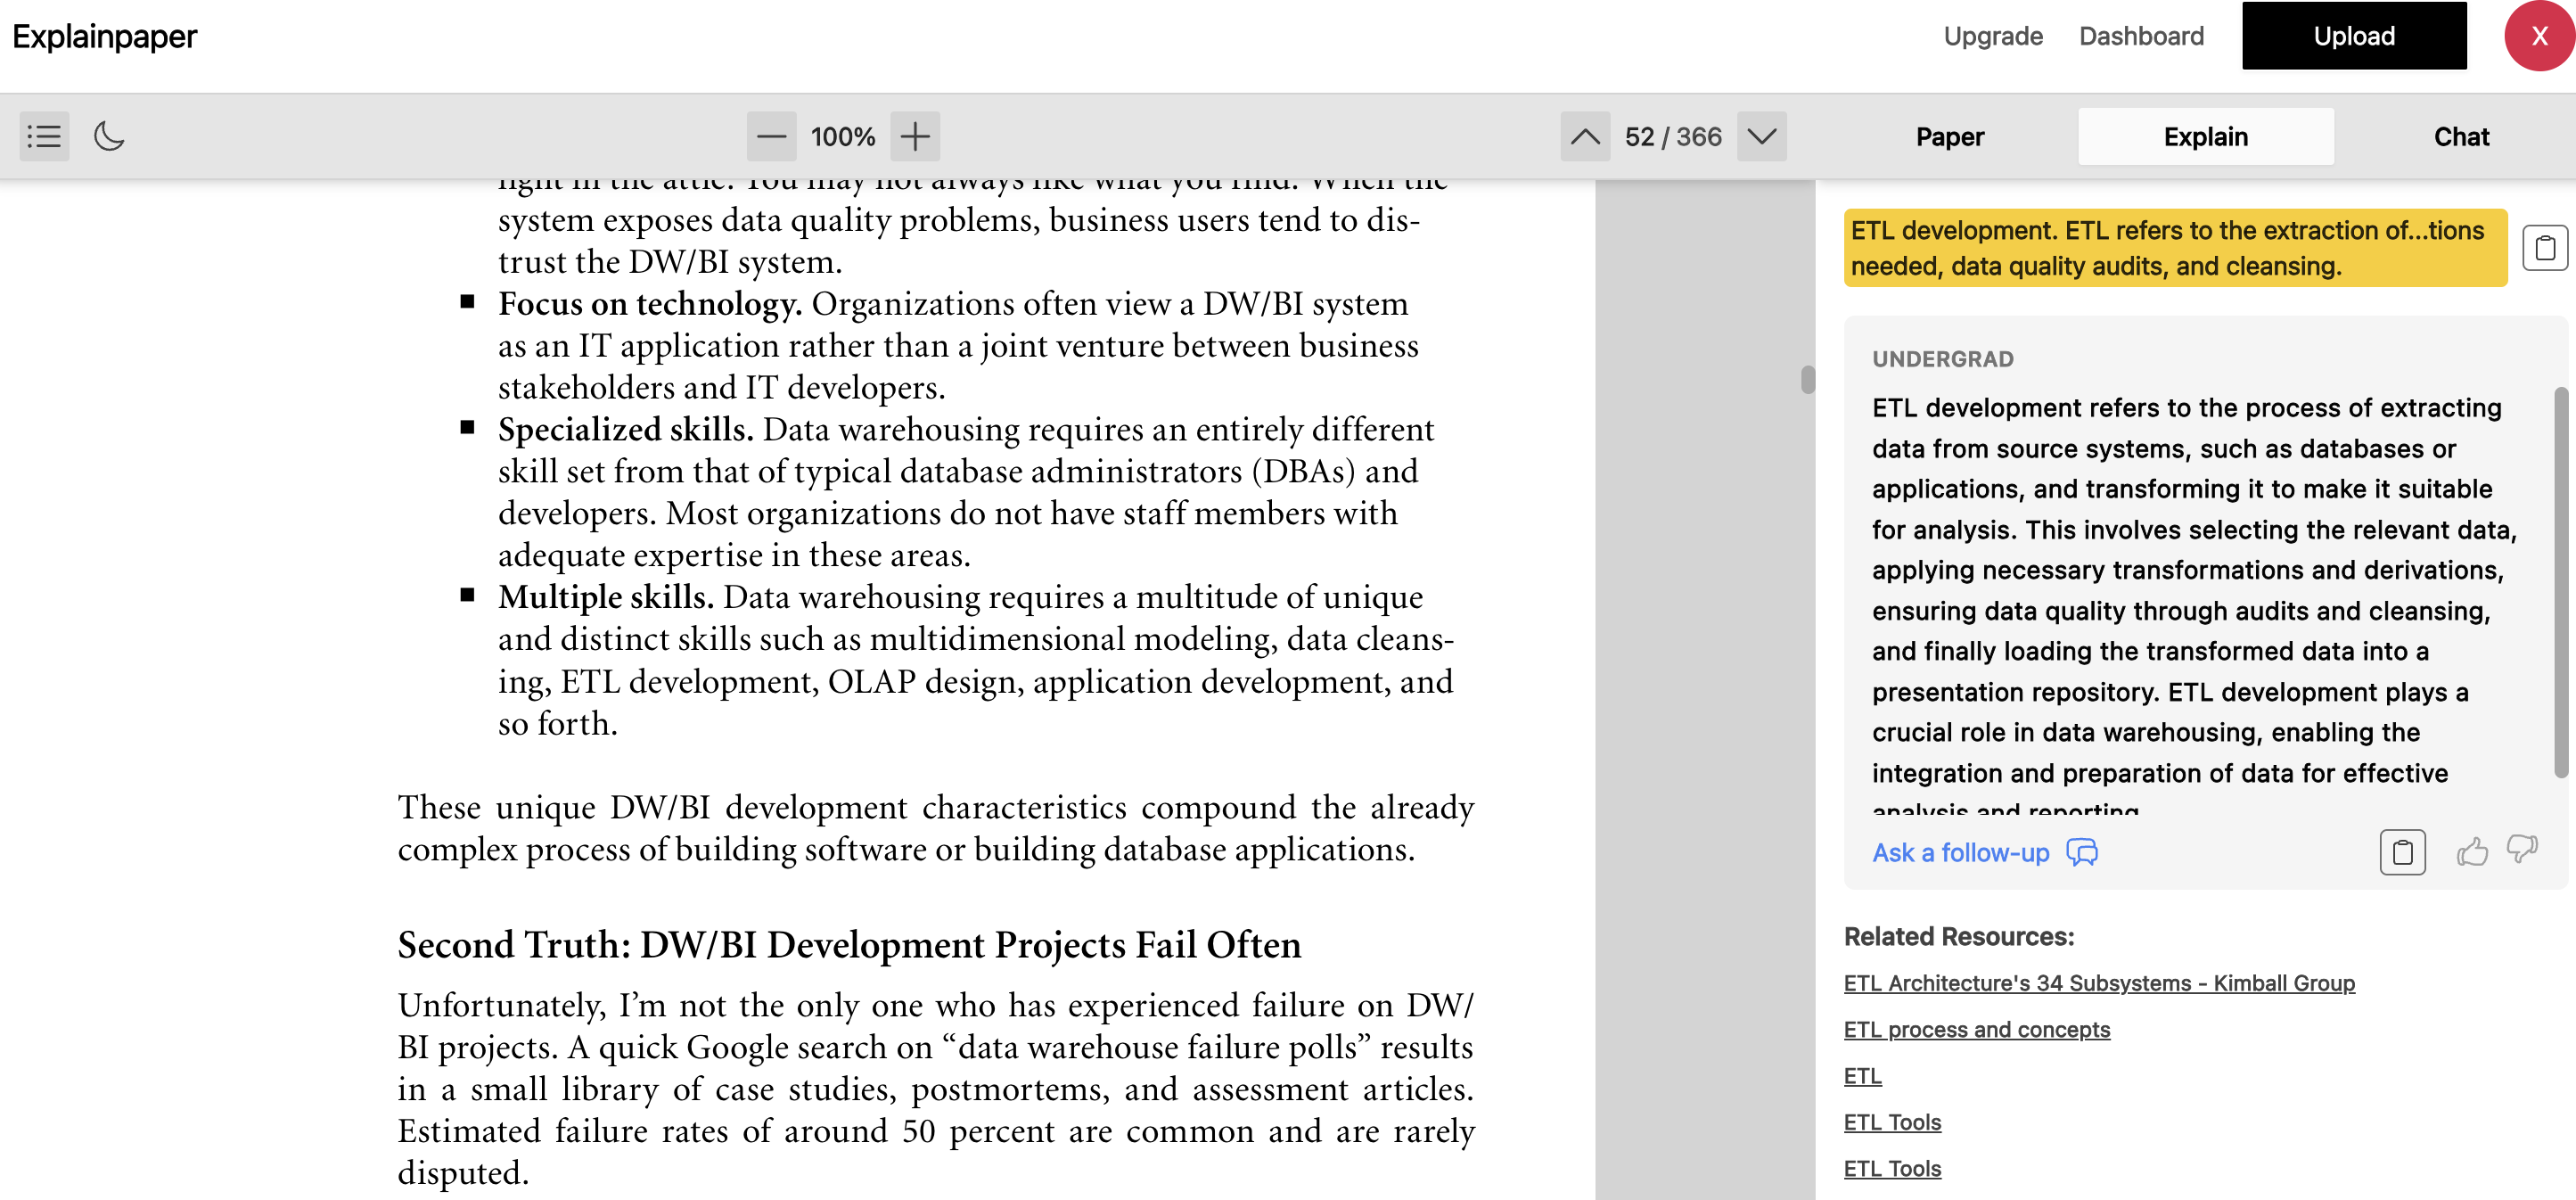
\includegraphics[width=0.9\linewidth]{Explainpaper_Example} 

}

\caption{Example of what Explainpaper can be used for}\label{fig:unnamed-chunk-12}
\end{figure}

\hypertarget{github-copilot}{%
\section{GitHub Copilot}\label{github-copilot}}

\href{https://github.com/features/copilot}{GitHub Copilot} is an AI developer tool that has gained significant recognition and was widely adopted within the programming community. Developed through a collaborative effort involving GitHub, OpenAI, and Microsoft, GitHub Copilot is a powerful tool that utilizes a generative AI model trained on extensive lines of code. Its primary function is to offer coding suggestions in multiple programming languages by interpreting natural language prompts.

\begin{figure}

{\centering 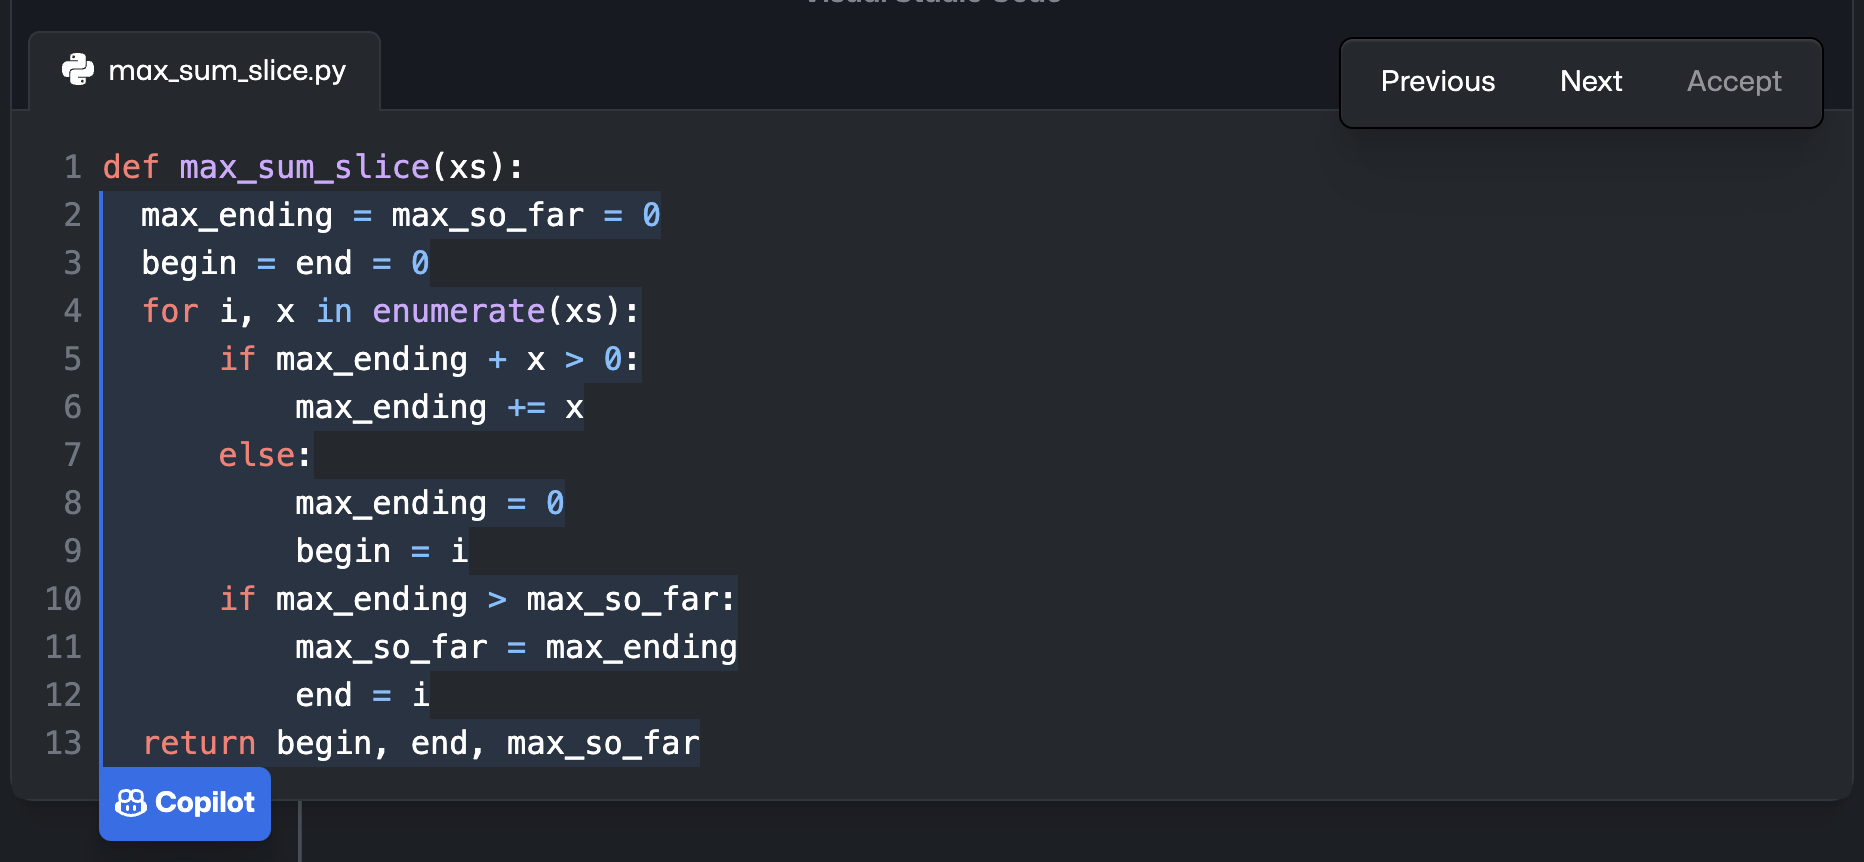
\includegraphics[width=0.95\linewidth]{GitHub_Copilot_Example} 

}

\caption{Example usage of GitHub Copilot}\label{fig:unnamed-chunk-13}
\end{figure}

\hypertarget{goblin-tools}{%
\section{Goblin Tools}\label{goblin-tools}}

\href{https://goblin.tools/}{Goblin Tool} offer a comprehensive solution for developers seeking guidance on difficult programming tasks. This tool utilizes its expertise to break down complex processes into manageable stages, which ensures that developers can follow a clear and structured path to successful implementation.

\begin{figure}

{\centering 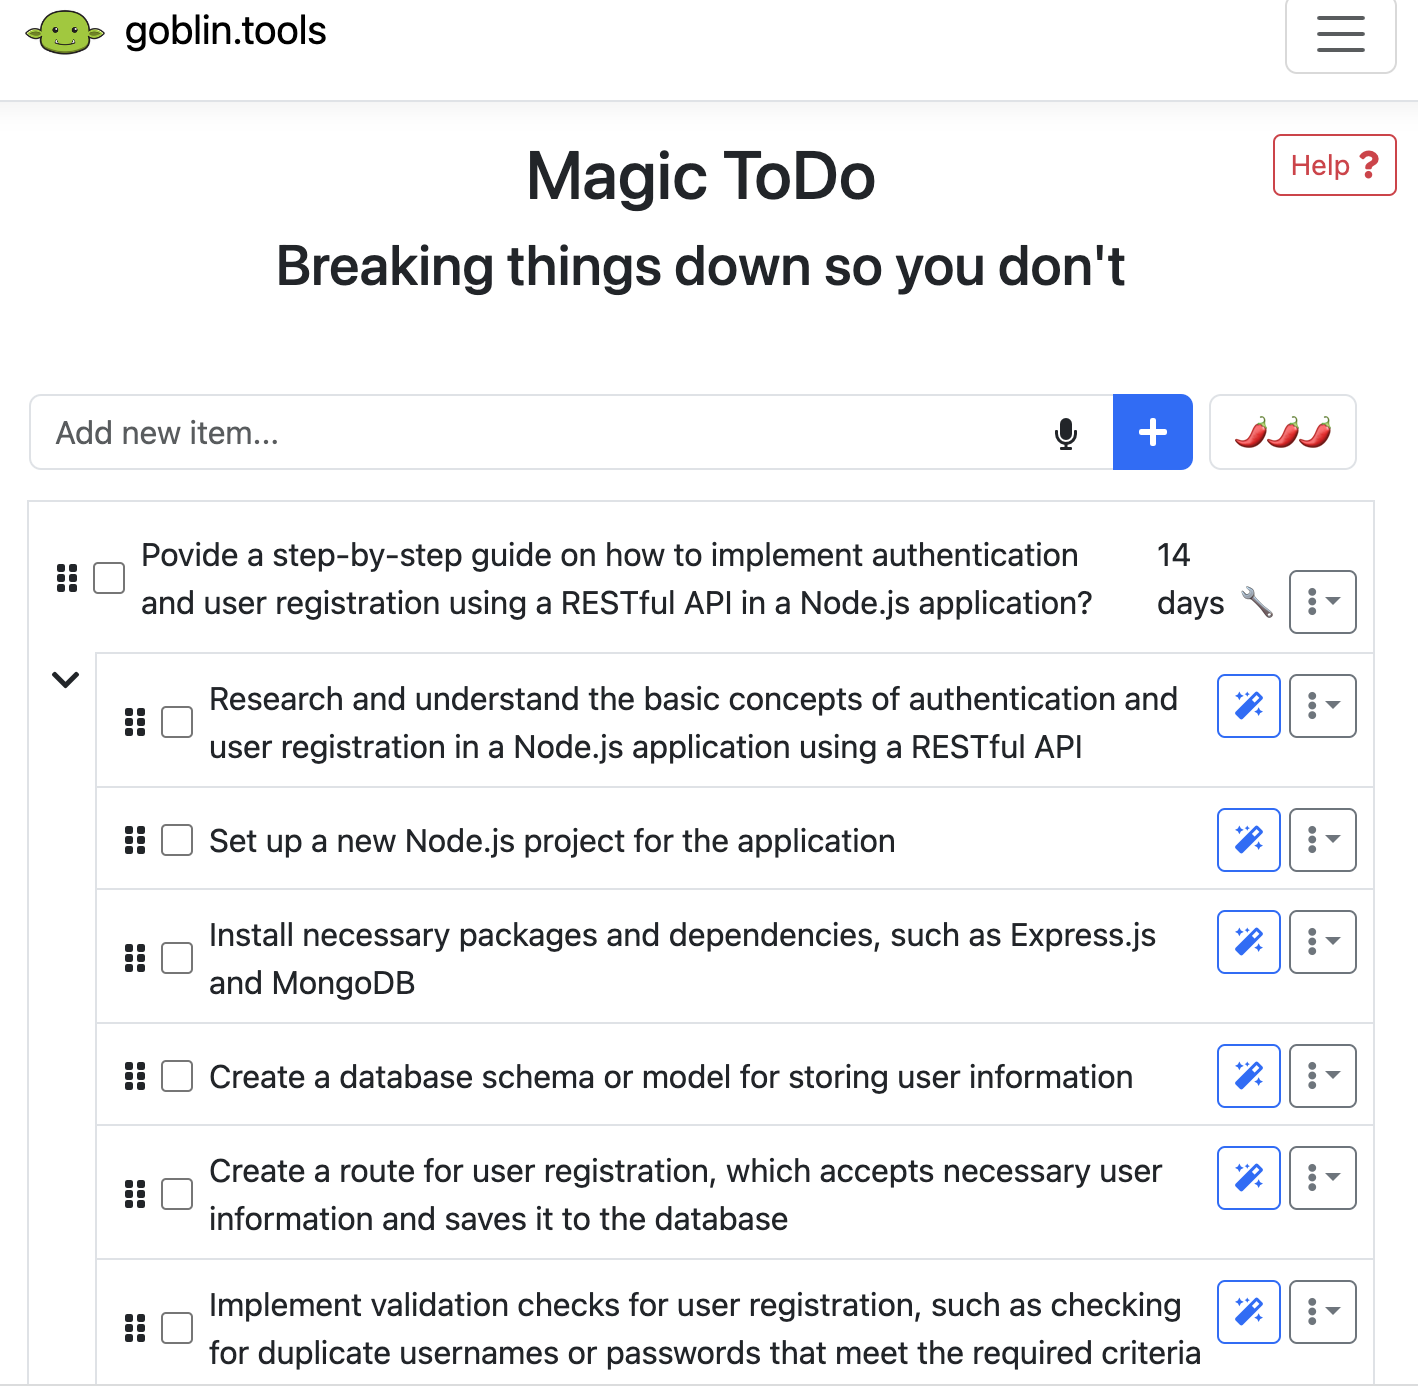
\includegraphics[width=0.7\linewidth]{Goblin_Tool_Example} 

}

\caption{Example of a programming task fed to Goblin Tool}\label{fig:unnamed-chunk-14}
\end{figure}

\hypertarget{dall-e}{%
\section{DALL-E}\label{dall-e}}

\href{https://labs.openai.com/}{DALL-E} is an advanced AI system developed by OpenAI that specializes in creating realistic images and art based on natural language descriptions. Users can provide text description of scenes, concepts or attributes and DALLE can translate these descriptions into images.

\begin{figure}

{\centering 
\includegraphics[width=0.7\linewidth]{Girl_with_a_pearlearrring_a_snake} 

}

\caption{"Girl with a pearl earring and a snake" by Johannes Vermeer}\label{fig:unnamed-chunk-15}
\end{figure}

\hypertarget{gen-1-runway-ml}{%
\section{Gen-1 Runway ML}\label{gen-1-runway-ml}}

\href{https://runwayml.com/}{Runway ML} allows users to transform text into video, create images from prompts, expand and re-image images, train custom AI models, manipulate videos, apply slow-motion effects, and so on.

\url{....}

\hypertarget{aiva}{%
\section{AIVA}\label{aiva}}

\href{https://www.aiva.ai/}{AIVA} is an AI tool designed to assist individuals in composing emotional and engaging soundtracks. It offers a range of predefined music styles like Modern, Pop, Rock, Jazz, etc. and to compose music. The platform offers a user-friendly interface that allows users to input specific parameters and preferences like style, mood and instrumentation and then generate original music that aligns with those criteria.

\begin{figure}

{\centering 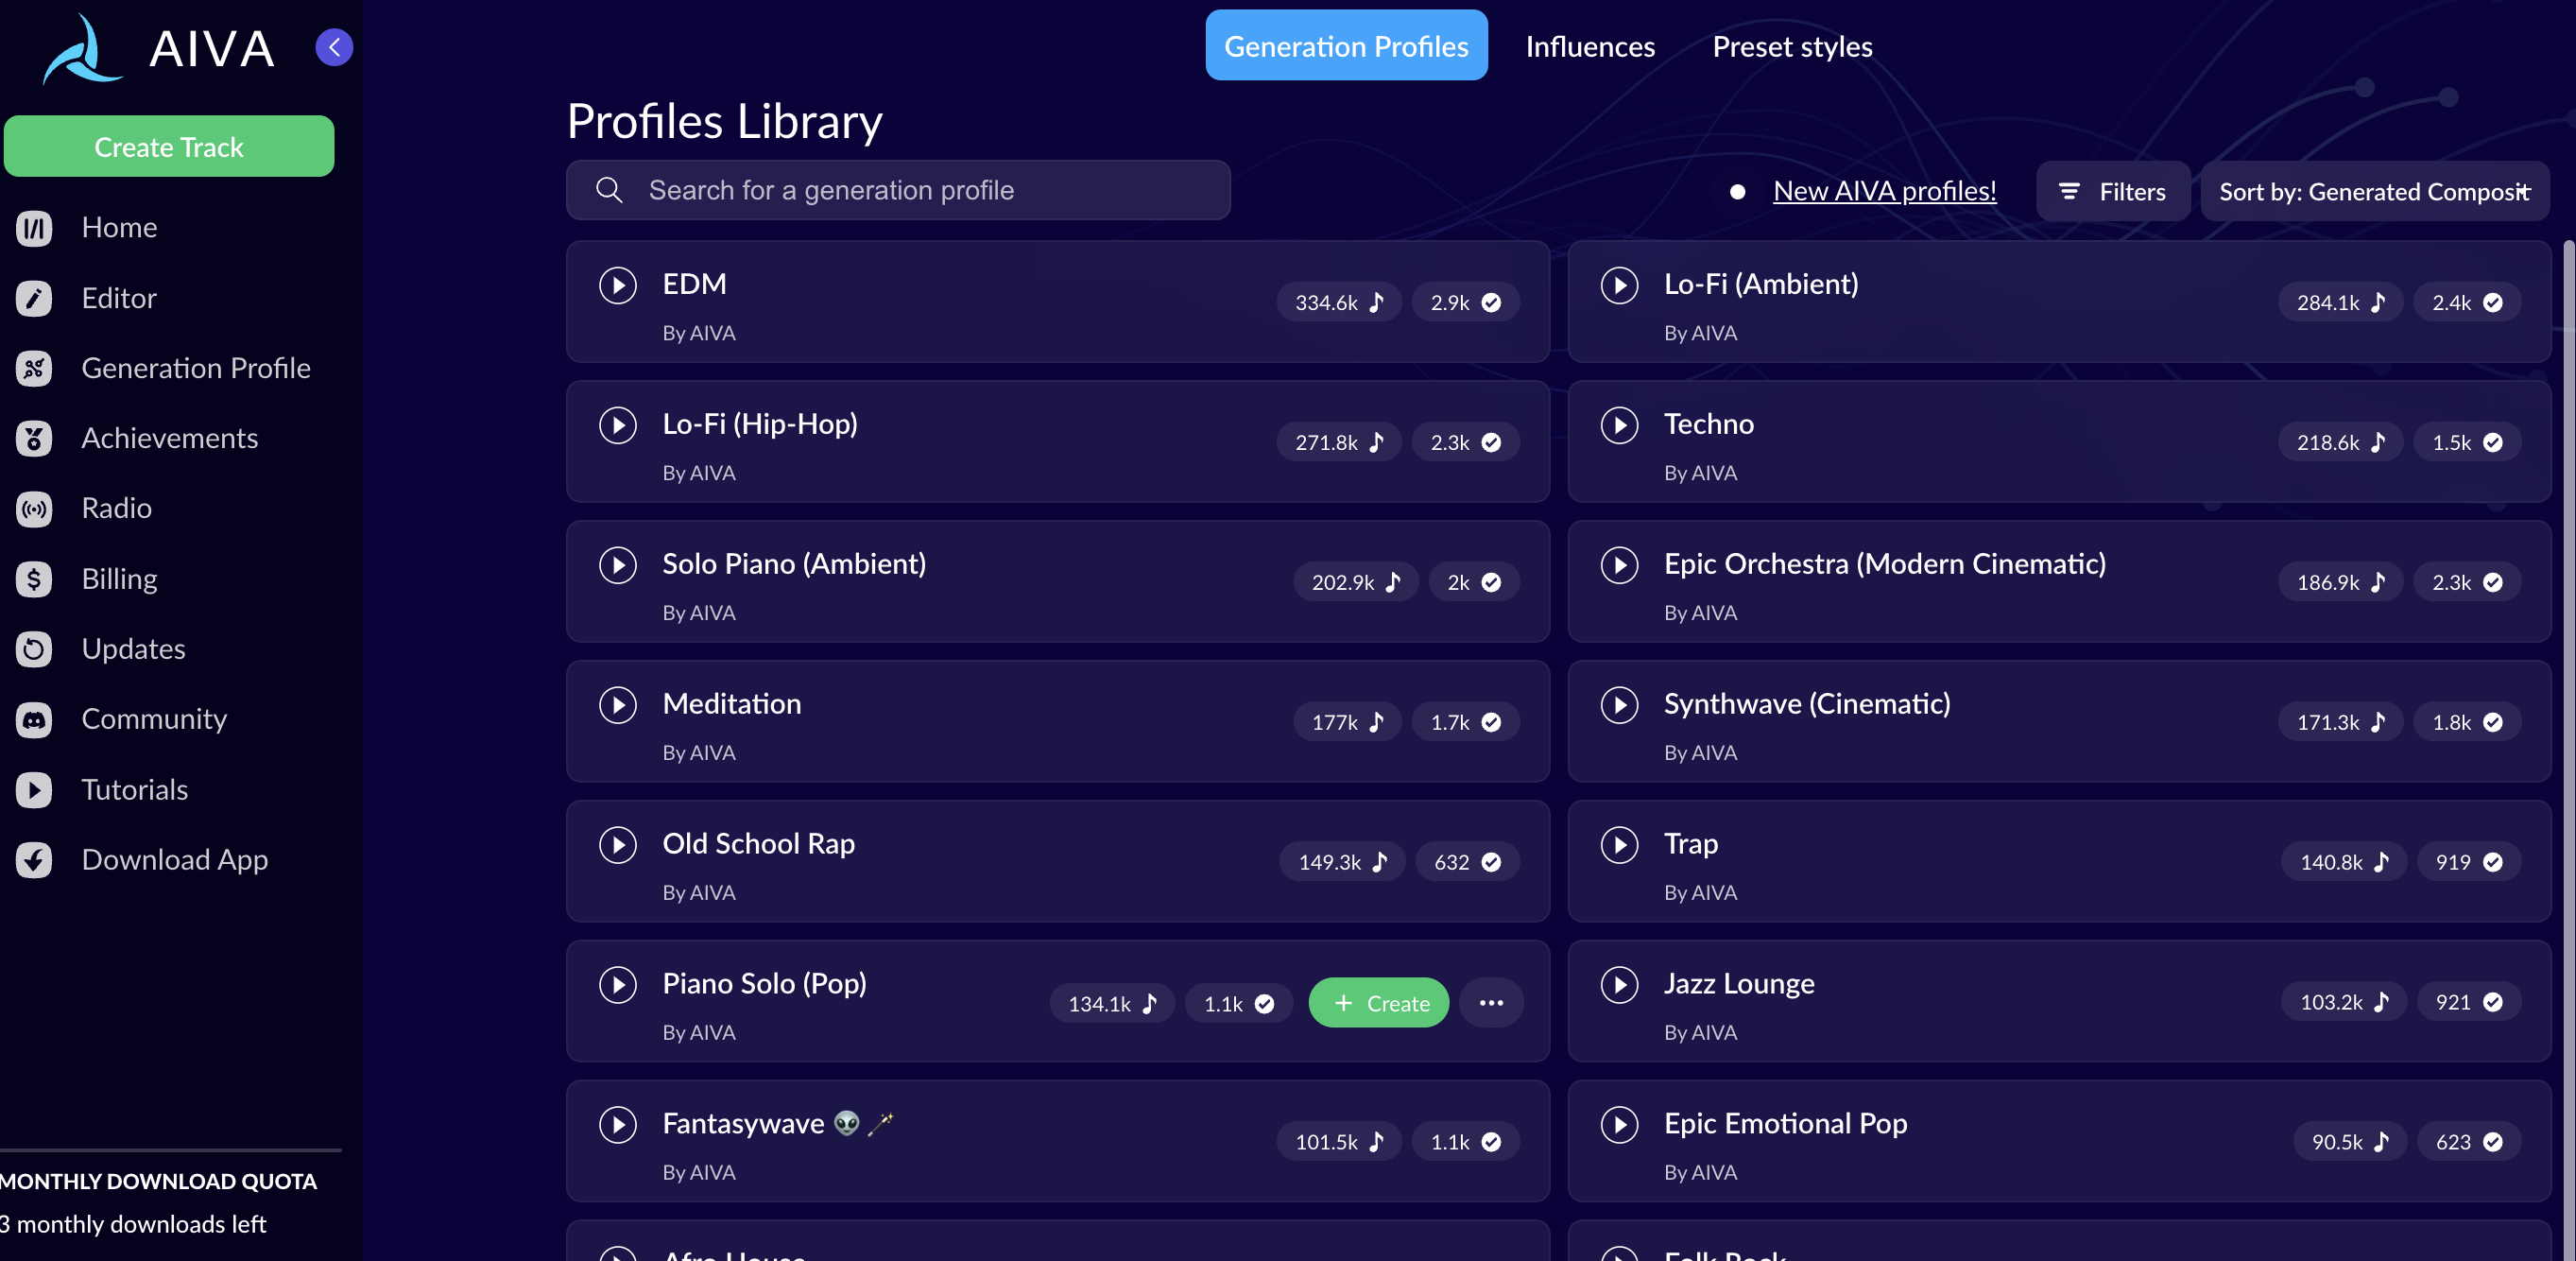
\includegraphics[width=0.95\linewidth]{AIVI_Dashboard} 

}

\caption{AIVI Dashboard}\label{fig:unnamed-chunk-17}
\end{figure}

\hypertarget{final-thoughts}{%
\chapter{Final Thoughts}\label{final-thoughts}}

The potential of Generative Artificial Intelligence is here. This report delves into the transformative influence of generative AI on business education, drawing insights from extensive faculty and staff interviews, exploring the capabilities of particular GenAI tools in higher education, and contextualizing them within the broader framework of university policies through the findings of the Generative AI Advisory (GAIA) committee.

The insights gathered from interviews with faculty and staff highlight the diversity of perspectives surrounding the use of AI tools in education. While some embrace its potential to reshape teaching and engagement, others raise valid concerns about academic integrity and the need for a balanced approach. The disparity between faculty members who embrace AI's potential and those who exhibit caution underscores the need for ongoing dialogue and collaboration. This will foster an environment where educators collectively shape the future of education, leveraging AI to elevate critical thinking, problem-solving, and creativity among students. As AI technologies continue to advance, it is imperative for the Ross School of Business to establish a collaborative discourse, promoting an atmosphere that allows for a unified approach to this groundbreaking technology.

Our investigation into the GAIA committee's findings underscores the University of Michigan's proactive stance in understanding and regulating the integration of generative AI into its educational framework. The emergence of a UMich-based ChatGPT competitor further exemplifies the institution's commitment to innovation and adaptability. It is essential for the University to continue fostering an environment that encourages experimentation and collaboration to effectively harness the potential of AI in a responsible and constructive manner.

This discussion of AI between educators and students alike at the University of Michigan must emphasize a balanced and informed approach to its integration---one that prioritizes a modern education for students while also maintaining academic integrity standards assumed by instructors. By establishing guidance that helps the community navigate the complexities of AI while also capitalizing on the vast opportunities that it presents within education, the Ross School of Business can initiate an era of education that is both enriched and elevated by the transformative power of generative AI.

\hfill\break

\end{document}
